% arara: pdflatex: { shell: yes, interaction: nonstopmode }
% arara: pythontex: {verbose: yes, rerun: modified }
% arara: pdflatex: { shell: yes, interaction: nonstopmode }
% arara: clean: { extensions: [ aux, blg, idx, ilg, ind, log, out, pytxcode, rel, toc ] }
% !arara: clean: { files: [ ans.tex, hint.tex] }

% arara: pdflatex
% arara: clean: { extensions: [ aux, blg, idx, ilg, ind, log, out, pytxcode, rel, toc ] }
% !arara: clean: { files: [ ans.tex, hint.tex] }


\documentclass[queueing-book-solution.tex]{subfiles}
%\externaldocument{queueing-book}

\opt{solutionfiles,check}{
\loadgeometry{tufte}
\Opensolutionfile{hint}
\Opensolutionfile{ans}
}

\begin{document}


\section{Level Crossing and Balance Equations}
\label{sec:level-cross-balance}

Consider a sample path\sidenote{The graph of the number of jobs in the system  obtained by simulation.} of $L:=\{\L\}$.
We say that the sample path \recall{up-crosses level $n$} at time $t$ when the  number of jobs $L$ in the system changes from $n$ to $n+1$ due to an arrival, in other words, when $L(t-)=n$ and $L(t)=n$. The sample path \recall{down-crosses level $n$} at time $t$ when $L$ changes from $n+1$ to $n$ due to a departure, that is, $L(t-)=n+1$ and $L(t)=n$.
Clearly, the number of up-crossings and down-crossings cannot differ by more than 1 at any time, because it is only possible to down-cross level $n$ after an up-crossing (or the other way around).
This simple idea will prove to be a key stepping stone in the analysis of queueing systems.

To establish this section's main result~\cref{eq:12}, we need a few definitions that are quite subtle, but we will provide intuitive and natural interpretations.\sidenote{They have practical significance too.}
After this, we will generalize the principle of level-crossing to \emph{balance equations} which allow us to deal with more general types of transitions.\sidenote{\cref{fig:summaries} at the end of this chapter provides  a graphical summary.}

\newthought{Let us say} that the system is in \emph{state}~$n$ at time $t$ when $L(t)=n$. Then define\sidenote{Note the $A_k-$; since $L(t)$ is right-continuous, we concentrate on what an \emph{arrival} sees just before it's arrival}
\begin{subequations}\label{eq:rates_}
\begin{equation}
 A(n,t) := \sum_{k=1}^{A(t)}\1{\L(A_k-) = n} = \sum_{k=1}^\infty \1{A_k \leq t}\1{\L(A_k-) = n}
\end{equation}
as the number of arrivals up to time $t$ that saw the system in state~$n$.\sidenote{\cref{ex:36},\cref{ex:38}}
\begin{marginfigure}%[t]
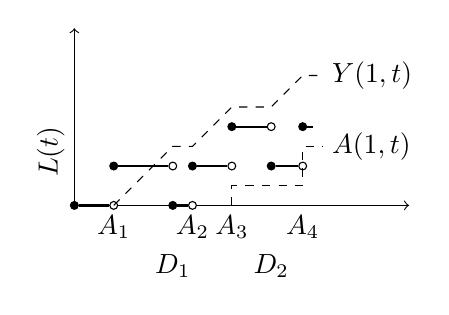
\begin{tikzpicture}[scale=0.5,
 open/.style={shape=circle, fill=white, inner sep=1pt, draw, node contents=},
 closed/.style={shape=circle, fill=black, inner sep=1pt, draw, node contents=},
]

%axis
\draw[->] (0,0) -- coordinate (x axis mid) (8.5,0);
\draw[->] (0,0) -- coordinate (y axis mid) (0,4.5);
%\node[below=0.2cm] at (x axis mid) {$t$};
\node[left=0.3cm, rotate=90] at (y axis mid) {$L(t)$};


\draw
node (0) at (0,0) [closed] {}
node (c1) at (1,0) [open] {};
\draw[thick] (0)--(c1);
\node[below] at (1,0) {$A_1$};

\draw
node (c2) at (1,1) [closed] {}
node (c3) at (2.5,1) [open] {};
\draw[thick] (c2)--(c3);
\node[below] at (2.5,-1) {$D_1$};

\draw
node (c2) at (2.5,0) [closed] {}
node (c3) at (3,0) [open] {};
\draw[thick] (c2)--(c3);
\node[below] at (3,0) {$A_2$};

\draw
node (c2) at (3,1) [closed] {}
node (c3) at (4,1) [open] {};
\draw[thick] (c2)--(c3);

\draw
node (c2) at (4,2) [closed] {}
node (c3) at (5,2) [open] {};
\draw[thick] (c2)--(c3);
\node[below] at (4,0) {$A_3$};

\draw
node (c2) at (5,1) [closed] {}
node (c3) at (5.8,1) [open] {};
\draw[thick] (c2)--(c3);
\node[below] at (5.,-1) {$D_2$};

\draw
node (c2) at (5.8,2) [closed] {}
node (c3) at (6.3,2) {};
\draw[thick] (c2)--(c3);
\node[below] at (5.8,0) {$A_4$};

\draw[dashed] (1,0)--(2.5, 1.5) -- (3, 1.5)--(4,2.5) --
(5, 2.5)--(5.8, 3.3)--(6.3, 3.3);
\node[right] at (6.3, 3.3) {$Y(1,t)$};

\draw[dashed] (4,0) -- (4,0.5)--(5.8, 0.5)--(5.8, 1.5)--(6.3, 1.5);
\node[right] at (6.3, 1.5) {$A(1,t)$};

\end{tikzpicture}
\footnotesize{\emph{We subtracted $1/2$ from the graph of $A(1,t)$, for otherwise this  overlaps with the graph of $Y$.}}
\end{marginfigure}
Next, let
\begin{equation}
 Y(n,t) := \int_0^t \1{\L(s) = n} \d s
\end{equation}
be the total time the system spends in state $n$ during $[0,t]$, and
\begin{equation} \label{eq:18}
 p(n,t) := \frac 1 t \int_0^t \1{\L(s) = n} \d s = \frac{Y(n,t)}t,
\end{equation}
\end{subequations}
be the fraction of time in state $n$ during $[0,t]$.



With the above definitions, we consider the limits,\sidenote{Again assuming they exist.}
\begin{align}\label{eq:p(n)}
 \lambda(n) &:= \lim_{t\to\infty} \frac{A(n,t)}{Y(n,t)}, &p(n) &=\lim_{t\to\infty} p(n,t),
\end{align}
as the arrival rate \emph{while} the system is in state~$n$, and the long-run fraction of time spent in state $n$.
To see the rationale behind this definition of $\lambda(n)$, recall that $A(t)/t$ is  the number of arrivals during $[0,t]$ divided by~$t$, while  $A(n,t)/Y(n,t)$ is the number of arrivals during $[0,t]$ that see $n$ jobs divided by the time the system contains $n$ jobs.


Similar to the definition for $A(n,t)$, let\sidenote{But now we take $D_k$, not $D_k-$.}
\begin{equation}\label{eq:102}
 D(n,t) := \sum_{k=1}^{D(t)} \1{\L(D_k) = n}  = \sum_{k=1}^\infty \1{D_k \leq t} \1{\L(D_k) = n}
 \end{equation}
 denote the number of departures up to time $t$ that\emph{ leave $n$
 customers behind}.
\begin{marginfigure}%[th]
\begin{tikzpicture}[scale=0.8,->,>=stealth',shorten >=1pt,auto,node distance=1.8cm,
 semithick]
 \node[state] (0) {$p(0)$} ;
 \node[state] (1) [right of=0] {$p(1)$};
 \node[state] (2) [right of=1] {$p(2)$};
% \node[state] (3) [right of=2] {}; %{$p(3)$};
% \node[state] (4) [right of=3] {$\cdots$};

\path
 (0) edge [bend left] node {$\lambda(0)$} (1)
 (1) edge [bend left] node {$\mu(1)$} (0)
 (1) edge [bend left] node {$\lambda(1)$} (2)
 (2) edge [bend left] node {$\mu(2)$} (1);
% (2) edge [bend left] node {$\lambda(2)$} (3)
% (3) edge [bend left] node {$\mu(3)$} (2)
% (3) edge [bend left] node {$\lambda(3)$} (4)
% (4) edge [bend left] node {$\mu(4)$} (3);

\draw[-, dotted, gray] (2.7,-2.)--(2.7,2.0) node[above, black] {level $1$};
\draw[->] (2,1.8) node[left] {$A(1,t)$} -- (3.5,1.8);
\draw[<-] (2,-1.8) node[left] {$D(1,t)$} --(3.5,-1.8) ;

\end{tikzpicture}
\end{marginfigure}
Then, define\sidenote{It is easy to get confused here: to leave $n$ jobs behind, the system must contain $n+1$ jobs just prior to the departure.}
\begin{equation*}
 \mu(n+1) := \lim_{t\to\infty} \frac{D(n,t)}{Y(n+1,t)},
\end{equation*}
as \emph{ the departure rate from state $n+1$}.

\newthought{The above definitions} may seem a bit abstract, but they have simple and practical interpretations.

Consider the sorting process of post parcels at a distribution center of a post-delivery company.
Each day tens of thousands of incoming parcels have to be sorted to their final destination.
Incoming parcels are deposited on a conveyor belt, and from there, they are carried to outlets, so-called chutes, from where the parcels are sent to a specific region of the Netherlands.
Employees pick up the parcels from the chutes and put the parcels in containers.
Sometimes parcels arrive a bit faster than the capacity of the employees and then a queue of parcels builds up in the chute.
When the chute overflows, parcels are directed to an overflow container and are sorted the next day.
The target of the sorting center is to deliver at least 99\% of the parcels within one day.

Suppose a chute can contain at most 20 parcels, say.
Then, each parcel on the belt that `sees' 20 parcels in its chute will be sent to the overflow container.
Clearly then, $A(20,t)/A(t)$ is the fraction of rejected parcels up to time~$t$.
For this reason,  sorting centers continuously track $A(20,\cdot)$ to adapt server capacity and control the fraction of rejected parcels.

For a second example, suppose it costs $w$ to have a job in queue for a unit of time.
%Then $ w n Y(n,t)$ is the total cost up to time $t$ to have $n$ jobs in queue, hence
The total cost up to time $t$ is then $w \sum_{n=0}^\infty n Y(n,t)$ and the average cost is
$w \sum_{n=0}^\infty n p(n,t)$.


\newthought{Continuing with the} theoretical discussion, observe that customers arrive and depart as single units.
Thus, if $\{T_k\}$ is the ordered set of arrival and departure epochs of the customers, then $L(T_k) = L(T_k-) \pm 1$.
But this implies that\sidenote{Think about this. This is simple, but has profound consequences.}
\begin{equation}\label{eq:97}
|A(n,t) - D(n,t)| \leq 1.
\end{equation}
From this observation it follows immediately that
\begin{equation}\label{eq:15}
 \lim_{t\to\infty} \frac{A(n,t)}t = \lim_{t\to\infty} \frac{D(n,t)}t.
\end{equation}
With this equation we obtain two nice identities.
The first we develop here, the other in~\cref{sec:poisson-arrivals-see}.

Clearly,\sidenote{Supposing the limits exist.} $\lim_{t\to\infty} A(n,t)/ t$ is the rate of arrivals that see the system in state $n$. With~\cref{eq:rates_} we see that
\begin{equation*}
\lim_{t\to\infty} \frac{A(n,t)}t = \lim_{t\to\infty} \frac{A(n,t)}{Y(n,t)}\frac{Y(n,t)}t = \lambda(n) p(n).
\end{equation*}
Similarly, the rate of jobs that leave $n$ jobs behind is
\begin{equation*}
\lim_{t\to\infty} \frac{D(n,t)}t = \lim_{t\to\infty} \frac{D(n,t)}{Y(n+1,t)}\frac{Y(n+1,t)}t = \mu(n+1) p(n+1).
\end{equation*}
Combining this with~\cref{eq:15} we arrive at the \recall{ level-crossing equations}\sidenote{This result is of fundamental importance in queueing (and inventory) theory.}
\begin{equation}\label{eq:12}
 \lambda(n) p(n) = \mu(n+1)p(n+1).
\end{equation}


\newthought{Suppose we can} specify\sidenote{In \cref{sec:mm1} and onward we will  model many queueing situations by making suitable choices for $\lambda(n)$ and $\mu(n)$.}
 the arrival and service rates $\lambda(n)$ and $\mu(n)$,
then we can easily compute the long-run fraction of time $p(n)$ that the system contains $n$ jobs.
To see this, rewrite~\cref{eq:12} as
\begin{equation}\label{eq:25}
 p(n+1) = \frac{\lambda(n)}{\mu(n+1)}p(n).
\end{equation}
A straightaway recursion then leads to
\begin{equation*}
 p(n+1) = \frac{\lambda(n)\lambda(n-1)\cdots \lambda(0)}{\mu(n+1)\mu(n)\cdots \mu(1)}p(0).
\end{equation*}
Thus, $p(n)$, $n\geq 1$, is just $p(0)$ times a constant, which is based on  arrival and service rates.

To determine $p(0)$ we can use the fact that the numbers $p(n)$ represent probabilities.
Hence, from the normalizing condition $\sum_{n=0}^\infty p(n)=1$, we get $p(0) = G^{-1}$ with
$G$ being the \emph{normalization constant}
\begin{equation} \label{eq:20}
G = 1+\sum_{n=0}^\infty \frac{\lambda(n)\lambda(n-1)\cdots\lambda(0)}{\mu(n+1)\mu(n)\cdots \mu(1)}.
\end{equation}

Finally, once we have $p(n)$, it is easy to compute  the time-average\sidenote{It is important to realize that this is not necessarily the same as what jobs see upon arrival.} number of jobs in the system and the long-run fraction of time the system contains at least $n$:
\begin{align*}
\E\L &= \sum_{n=0}^\infty n p(n), & \P{\L \geq n} &= \sum_{i=n}^\infty p(i).
\end{align*}


\newthought{It is important} to realize that the level-crossing argument cannot always be used, as it is not always possible to split the state space into two disjoint parts by `drawing a line' between two states.
For a more general approach, we focus on a single state and count how often this state is entered and left.
\begin{marginfigure}
\begin{tikzpicture}[scale=0.8,->,>=stealth',shorten >=1pt,auto,node distance=1.8cm,
 semithick]
% \node[state] (0) {$p(0)$} ;
 \node[state] (1) [right of=0] {$p(1)$};
 \node[state] (2) [right of=1] {$p(2)$};
 \node[state] (3) [right of=2] {$p(3)$};
% \node[state] (4) [right of=3] {$\cdots$};

\draw[dashed] (3.4,-1.8) rectangle (5.6,1.8);

\path
% (0) edge [bend left] node {$\lambda(0)$} (1)
% (1) edge [bend left] node {$\mu(1)$} (0)
 (1) edge [bend left] node[fill=white] {$\lambda(1)$} (2)
 (2) edge [bend left] node[fill=white] {$\mu(2)$} (1)
 (2) edge [bend left] node[fill=white] {$\lambda(2)$} (3)
 (3) edge [bend left] node[fill=white] {$\mu(3)$} (2);
 % (3) edge [bend left] node[above] {$\lambda(3)$} (4)
 % (4) edge [bend left] node[below] {$\mu(4)$} (3);
\end{tikzpicture}
\end{marginfigure}
Specifically, define $I(n,t) = A(n-1,t) + D(n,t)$ as the number of times the queueing process enters state $n$ either due to an arrival from state $n-1$ or due to a departure leaving $n$ jobs behind. Similarly,  $O(n,t) = A(n,t) + D(n-1,t)$ counts how often state $n$ is left either by an arrival (to state $n+1$) or a departure (to state $n-1$).


Just like~\eqref{eq:97}, it is evident that $|I(n,t)-O(n,t)|\leq 1$, and this implies\sidenote{~\cref{ex:79}}
\begin{equation}\label{eq:104}
 \lambda(n-1)p(n-1)+\mu(n+1)p(n+1) = (\lambda(n)+\mu(n))p(n).
\end{equation}
These equations hold for any $n\geq 1$ and are known as the \recall{balance equations}.
We will use these equations to analyze queueing networks.




\begin{exercise}\label{ex:36}
 Show that $A(t) =\sum_{n=0}^\infty A(n,t)$.
\begin{solution}
 \begin{equation*}
A(t) = \sum_{k=1}^\infty \1{A_k \leq t} = \sum_{k=1}^\infty \sum_{n=0}^\infty \1{\L(A_k-) = n} \1{A_k \leq t}  = \sum_{n=0}^\infty A(n,t).
 \end{equation*}
\end{solution}
\end{exercise}

\begin{exercise} \label{ex:38}
If $\lambda>\delta$ can it happen that $ \lim_{t\to\infty} A(n,t)/t > 0$ for some (finite) $n$?
\begin{solution}
 If $\lambda > \delta$, then $L(t)\to\infty$.
 But then there must be a last time, $s$ say, that $L(s) = n+1$, and $L(t) > n+1$ for all $t>s$.
 Hence, after time $s$ no job will see the system with $n$ jobs.
 Thus $A(n,t) = A(n,s)$ for all $t>s$.
As this is  finite, $\lim_{t\to\infty}A(n,t)/t=0$.
\end{solution}
\end{exercise}

 \begin{exercise} \label{ex:111}
Consider the following (silly) queueing process.\marginpar{What acronym would describe this queueing situation?}
 At times $0, 2,4, \ldots$ customers arrive, each customer requires $1$ unit of service, and there is one server.
 Find an expression for $A(n,t)$, when $L(0)=0$.
\begin{solution}
 It is the $D/D/1$ queue. Next, $A_{k} = 2(k-1)$ as jobs arrive at $t=0, 2, 4, \ldots$
 We also know that $L(s)=1$ if $s\in [2k, 2k+1)$ and $L(s)=0$ for $s\in[2k-1, 2k)$ for $k=0, 1, 2, \ldots$.
 Thus, $L(A_k-) = L(2k-)=0$.
 Hence, $A(0,t) \approx t/2$ for $t\gg 0$, and $A(n,t)=0$ for $n\geq 1$.
\end{solution}
\end{exercise}


\begin{exercise} \label{ex:112}
 Find\marginpar{Continuation of~\cref{ex:111}}
 an expression for $Y(n,t)$.
\begin{solution}
Observe that the system never contains
 more than 1 job. Hence, $Y(n,t)=0$ for all $n\geq 2$. Then we see that
 $Y(1,t) = \int_0^t \1{\L(s) = 1}\d s$. Now observe that for our
 queueing system $L(s)=1$ for $s\in[0,1)$, $L(s)=0$ for
 $s\in[1,2)$, $L(s)=1$ for $s\in[2,3)$, and so on. Thus, when
 $t<1$, $Y(1,t)=\int_0^t \1{\L(s)=1} \d s = \int_0^t 1\d s = t$.
 When $t\in[1,2)$,
 \begin{equation*}
 L(t)=0 \implies \1{\L(t)=0} \implies Y(1,t) \text{ does not change}.
 \end{equation*}
Continuing to $[2,3)$ and so on gives
 \begin{equation*}
 Y(1,t) =
 \begin{cases}
 t & t\in[0,1), \\
 1 & t\in[1,2), \\
 1+(t-2) & t\in[2,3), \\
 2 & t\in[3,4), \\
 2+(t-4) & t\in[4,5), \\
 \end{cases}
 \end{equation*}
 and so on. Since $Y(n,t)=0$ for all $n\geq 2$, $L(s) = 1$ or
 $L(s)=0$ for all $s$, therefore,
 \begin{equation*}
 Y(0,t) = t-Y(1,t).
 \end{equation*}
\end{solution}
\end{exercise}

\begin{exercise} \label{ex:113}
Compute\marginpar{Continuation of~\cref{ex:112}}
$p(n)$ and $\lambda(n)$.
\begin{solution}
 From the other exercises:
 \begin{align*}
 \lambda(0) &\approx \frac{A(0,t)}{Y(0,t)} \approx \frac{t/2}{t/2} = 1, \\
 \lambda(1) &\approx \frac{A(1,t)}{Y(1,t)} \approx \frac{0}{t/2} = 0, \\
 p(0) &\approx \frac{Y(0,t)}{t} \approx \frac{t/2}{t} = \frac 1 2, \\
 p(1) &\approx \frac{Y(1,t)}{t} \approx \frac{t/2}{t} = \frac 1 2.
 \end{align*}
For the rest $\lambda(n) = 0$, and $p(n)=0$, for $n\geq 2$.
\end{solution}
\end{exercise}


\begin{exercise}\label{ex:4}
Compute\marginpar{Continuation of~\cref{ex:113}}
$D(n,t)$ and $\mu(n+1)$ for $n\geq 0$.
\begin{solution}
 $D(0,t) = \sum_{k=1}^\infty\1{D_k\leq t, L(D_k)=0}$. From the graph of $\{\L(s)\}$ we see that all jobs leave an empty system behind. Thus, $D(0,t) \approx t/2$, and $D(n,t)=0$ for $n\geq 1$. With this, $D(0,t)/Y(1,t) \sim (t/2)/(t/2) = 1$, and so,
 \begin{equation*}
 \mu(1) = \lim_{t\to\infty} \frac{D(0,t)}{Y(1, t)} = 1,
 \end{equation*}
and $\mu(n) = 0$ for $n\geq2$.
\end{solution}
\end{exercise}



\begin{exercise}\label{ex:l-110}
 Compute\marginpar{Continuation of~\cref{ex:4}} $\lambda(n) p(n)$ for $n\geq 0$, and check $\lambda(n) p(n) = \mu(n+1) p(n+1)$.
\begin{solution}
 $\lambda(0)p(0)=1\cdot 1/2 = 1/2$, $\lambda(n)p(n)= 0$ for $n>1$, as $\lambda(n)=0$ for $n>0$.

From~\cref{ex:4}, $\mu(1)=1$, hence $\mu(1) p(1) = 1\cdot 1/2 = 1/2$. Moreover, $\mu(n)=0$ for $n\geq 2$.

Clearly, for all $n$ we have $\lambda(n)p(n)= \mu(n+1)p(n+1)$.

\end{solution}
\end{exercise}


\begin{exercise}\label{ex:l-111}
 Derive $\E\L = \sum_{n=0}^\infty n p(n)$ from~\cref{eq:46}.
\begin{solution}
Noting that %As $L(s)$ counts the number of jobs in the system at time $s$ (thus $L(s)$ is an integer),
$L(s) = \sum_{n=0}^\infty n\, \1{\L(s) = n}$,
%With this we can write for the time-average number of jobs in the system
\begin{equation*}
\frac 1 t \int_0^t L(s) \d s = \frac 1 t \int_0^t \left(\sum_{n=0}^{\infty} n\, \1{\L(s) = n}\right) \d s
= \sum_{n=0}^{\infty} \frac n t \int_0^t \1{\L(s) = n} \d s,
\end{equation*}
Now apply~\cref{eq:18}.
\end{solution}
\end{exercise}







\begin{exercise}\label{ex:67}
Consider\marginpar{When level-crossing arguments can be applied, the analysis often becomes quite easy.}
a single server that serves one queue and serves only in batches of 2 jobs at a time (so never 1 job or more than 2 jobs).  At most 3 jobs fit in the system.
\marginpar{What is the acronym for this system?}
 Single jobs arrive as a Poisson process with $\lambda$.
Due to blocking, we take $\lambda(n) = \lambda$ for $n<3$ and $\lambda(n)=0$ for $n\geq 3$.
The batch service times are exponentially distributed with mean $1/\mu$, so that  by the memoryless property, $\mu(n) = \mu$.

Make a graph of the state-space and show, with arrows, the transitions that can occur and  use level-crossing arguments to express the steady-state probabilities $p(n), n=0,\ldots, 3$ in terms of $\lambda$ and $\mu$.
\begin{solution}
It is the $M/M^2/1/3$ queue.

\begin{tikzpicture}[scale=1,->,>=stealth',shorten >=1pt,auto,node distance=2.8cm,
 semithick]
\node[state] (0) {$0$};
\node[state] (1) [right of=0] {$1$};
\node[state] (2) [right of=1] {$2$};
\node[state] (3) [right of=2] {$3$};

\path
(0) edge [bend left] node[above] {$\lambda$} (1)
(1) edge [bend left] node[above] {$\lambda$} (2)
(2) edge [bend left] node[above] {$\lambda$} (3)
(3) edge [bend left] node[below] {$\mu$} (1)
(2) edge [bend left] node[below] {$\mu$} (0);

\draw[-, dotted, gray] (4,-2.)--(4,2.0) node[above, black] {level $1$};
\end{tikzpicture}

With level-crossing:
 \begin{align*}
 \lambda p(0) &= \mu p(2), \quad\text{the level between 0 and 1,}\\
 \lambda p(1) &= \mu p(2) +\mu p(3), \quad\text{see level 1,}\\
 \lambda p(2) &= \mu p(3), \quad\text{the level between 2 and 3.}\\
 \end{align*}
 Solving this in terms of $p(0)$ gives $p(2) = \rho p(0)$, $p(3) = \rho p(2) = \rho^2p(0)$, and
 \begin{equation*}
 \lambda p(1) = \mu(p(2) + p(3)) = \mu (\rho + \rho^2) p(0) = (\lambda + \lambda^2/\mu) p(0),
 \end{equation*}
hence $p(1) = p(0)(\mu + \lambda)/\mu$.
\end{solution}
\end{exercise}

\begin{exercise}\label{ex:79}
Show \cref{eq:104} from  $|I(n,t)-O(n,t)|\leq 1$.
\end{exercise}
\begin{solution}
\begin{equation*}
\lim_{t\to\infty} \frac{I(n,t)}t = \lim_{t\to\infty} \frac{A(n-1,t)}t + \lim_{t\to\infty} \frac{D(n,t)}t = \lambda(n-1) p(n-1) +
\mu(n+1) p(n+1)
\end{equation*}
and
\begin{equation*}
\lim_{t\to\infty} \frac{O(n,t)}t = \lim_{t\to\infty} \frac{A(n,t)}t + \lim_{t\to\infty} \frac{D(n-1,t)}t = \lambda(n) p(n) +
\mu(n) p(n)
\end{equation*}
\end{solution}

\opt{solutionfiles}{\Closesolutionfile{hint}
\Closesolutionfile{ans}
\loadgeometry{normal}
\input{hint}
\input{ans}
}

\end{document}


%%% Local Variables:
%%% mode: latex
%%% TeX-master: t
%%% End:
